\documentclass{beamer}

\usepackage{amsmath}
\usepackage{amsthm}
\usepackage{float}
\usepackage{graphicx}
\usepackage{color}
\usepackage{url}
\usepackage{listings}
\usepackage{../cppenv}

\newcommand{\red}[1]{\textcolor{red}{#1}}
\newcommand{\blue}[1]{\textcolor{blue}{#1}}
\newcommand{\gray}[1]{\textcolor{gray}{#1}}

\newcommand{\ttt}[1]{\texttt{#1}}
\newcommand{\bluett}[1]{\blue{\ttt{#1}}}
\newcommand{\redtt}[1]{\red{\ttt{#1}}}

\newenvironment{question}{\begin{alertblock}{Question}}{\end{alertblock}}
\theoremstyle{definition}
\newtheorem{thm}{Theorem}
\newtheorem{dfn}{Definition}

\usetheme{Warsaw}
\usecolortheme{wolverine}

\title{CS100 Recitation 4}
\author{Dinghao Cheng}
\institute{Special thanks: Gkxx}
\date{March 15, 2022}

\begin{document}

\begin{frame}
    \titlepage
\end{frame}

\AtBeginSection[]{
    \begin{frame}{Contents}
        \tableofcontents[currentsection]
    \end{frame}
}

\section{Pointers and Arrays}

\subsection{Basic Knowledge}

\begin{frame}{`\ttt{*}' and `\ttt{\&}'}
    \begin{itemize}
        \item In declaration statements, `\ttt{*}' is the \blue{pointer specifier}.
        \item In an expression, `\ttt{*}' is the \blue{dereference operator}.
        \item For a pointer \ttt{p}, \ttt{*p} is \blue{dereferencing the pointer}, which returns the \blue{object} that \ttt{p} points to.
        \item In an expression, `\ttt{\&}' is the \blue{address-of operator}, which takes the address of the operand.
    \end{itemize}
\end{frame}

\begin{frame}[fragile]{Conversion from Array to Pointer}
    \begin{cpp}
int a[10];
int *p1 = a;
int *p2 = &a[0];
    \end{cpp}
    \begin{itemize}
        \item The array can be \blue{implicitly converted} to the address of the first element,
        \item \red{but pointer and array are different types!}
        \pause
        \item \ttt{p1 + 3} is the same as \ttt{\&p1[3]}.
    \end{itemize}
\end{frame}

\begin{frame}[fragile]{Array and Pointer......}
    \begin{itemize}
        \item What's wrong with this code snippet?
        \begin{cpp}
char* str=(char*)malloc(sizeof(char)*10000);
memset(str,0,sizeof(str));
        \end{cpp}
        \pause
        \item Consider: What does \texttt{sizeof(str)} return?
    \end{itemize}
\end{frame}

\begin{frame}[fragile]{How to find bugs easily?}
    \begin{cpp}
char* str=(char*)malloc(sizeof(char)*10000);
memset(str,0,sizeof(str));
    \end{cpp}
    \begin{itemize}
    \item \blue{Use Warnings!!!}
    \pause
    \item \texttt{-Wpedantic -Wall -Wextra}
    \end{itemize}
    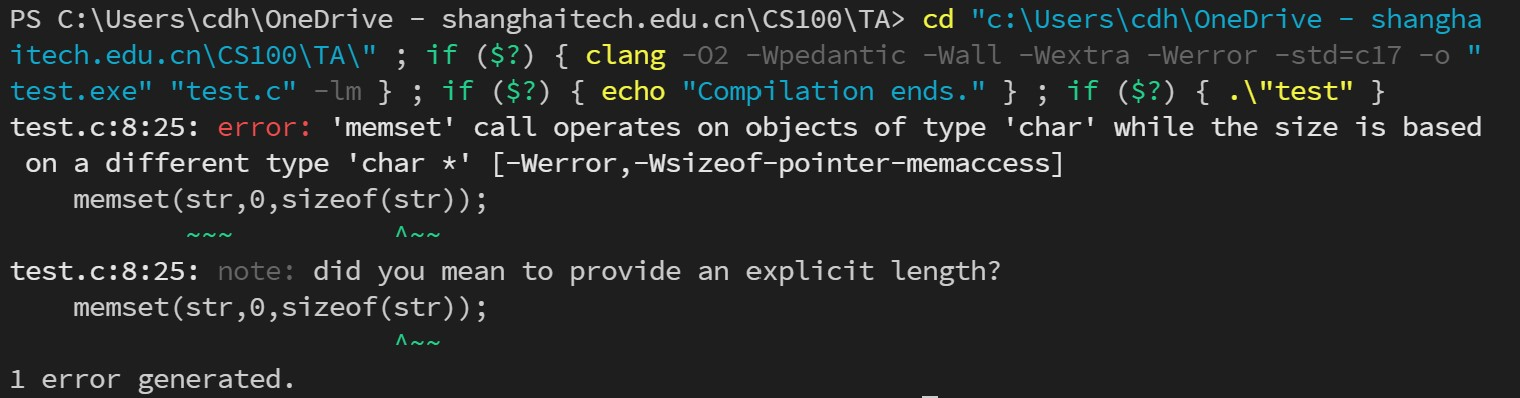
\includegraphics[width=\linewidth]{pic1.jpg}
\end{frame}

\begin{frame}[fragile]
    \begin{thm}
        Suppose \ttt{p} is defined to be a pointer of type \ttt{T *} and \ttt{i} is an integer. Then \ttt{(p + i)} is the address obtained by shifting from \ttt{p} by \ttt{i * }\bluett{sizeof}\ttt{(T)} bytes.
    \end{thm}
    \pause
    \begin{cpp}
int a[10];
int *pi = a;
int (*pa)[10] = &a;
printf("%p, %p\n", pi, pa);
printf("%p, %p\n", pi + 3, pa + 3);
    \end{cpp}
\end{frame}

\begin{frame}{Value of Pointer}
    At any time, a pointer might be:
    \begin{enumerate}
        \item pointing to an object.
        \item pointing to the location just immediately past the end of an object.
        \item \redtt{NULL}, indicating that it is not pointing to any object.
        \item pointing to nowhere \red{(invalid)}; values other than the preceding three are invalid.
    \end{enumerate}
\end{frame}

\begin{frame}{Value of Pointer}
    \begin{itemize}
        \item A pointer has \red{invalid} value after \blue{default initialization}.
        \item A pointer is \redtt{NULL} after \blue{value initialization}.
        \pause
        \item Default-initialized pointers that point to nowhere are called \blue{wild pointers}.
        \item Pointers also have \red{invalid} value after being \ttt{free}d. This is called a \blue{dangling pointer}.
    \end{itemize}
\end{frame}

\begin{frame}[fragile]{Value of Pointer}
    \begin{thm}
        A pointer is \blue{dereferencable} if and only if it is pointing to an object.
    \end{thm}
    \begin{itemize}
        \item Taking an invalid address as the value of a pointer is okay,
        \item but any attempt to dereference an \blue{undereferencable} pointer is severe runtime-error.
        \pause
        \item \begin{cpp}
int a[10];
int (*p)[10] = &a;
        \end{cpp}
        \ttt{p + 3} is okay, but \ttt{*(p + 3)} and \ttt{p[3]} cause runtime-error!
    \end{itemize}
\end{frame}

\subsection{Dynamic Memory}

\begin{frame}[fragile]{Magic Square}
    \begin{cpp}
int **magicSquare(int n) {
  int **p = malloc(sizeof(int *) * n);
  for (int i = 0; i < n; ++i)
    p[i] = malloc(sizeof(int) * n);
  // What is the value of each p[i][j] now?
  /* Fill the magic square. */
  return p;
}
void freeMagicSquare(int **p, int n) {
  for (int i = 0; i < n; ++i)
    free(p[i]);
  free(p);
}
    \end{cpp}
\end{frame}

\begin{frame}[fragile]{Magic Square}
    How many problems are there?
    \begin{cpp}
int **magicSquare(int n) {
  int p[n][n];
  // Fill the magic square.
  return p;
}
    \end{cpp}
    \pause
    \begin{itemize}
        \item VLA is not recommended in C and forbidden in C++.
        \item \ttt{p} is a \blue{local variable} of the function, which is destroyed immediately the function ends.
        \item \ttt{int [n][n]} can be converted to \ttt{int (*)[n]} naturally, but then the conversion from \ttt{int (*)[n]} to \ttt{int **} is severe runtime-error! (We will talk about this later.)
    \end{itemize}
\end{frame}

\begin{frame}[fragile]{Usage of \ttt{free}}
    \ttt{free(p)} frees the memory that starts at the address pointed by \ttt{p}.
    \begin{itemize}
        \item If \ttt{p} is not pointing to some memory that is dynamically allocated, \ttt{free(p)} causes runtime-error.
        \item The system knows the size of the memory, and the entire piece of memory will be freed. You \red{cannot free only a part of it}.
        \item Any attempt to free only a part of a piece of memory causes runtime-error.
    \end{itemize}
\end{frame}

\section{C-style Strings}

\begin{frame}{Definition}
    \begin{dfn}
        A group of characters stored in contiguous memory terminated with a null character \ttt{`\textbackslash 0'} is a C-style string.
    \end{dfn}
    \pause
    \begin{itemize}
        \item \red{The value of a \ttt{char} variable is exactly the ASCII of the character it represents.}
        \item ASCII of \ttt{`\textbackslash 0'}: \blue{0}.
        \item \ttt{char str[6] = "Hello";}
        \item The \blue{length} of a string is the number of real characters in the string, in which the null character is not counted.
    \end{itemize}
\end{frame}

\begin{frame}{The \ttt{string.h} Library}
    Make sure you know them before using!
    \begin{itemize}
        \item \ttt{strlen(s)} returns the length of the string \ttt{s}. The \ttt{return}ed value is of type \ttt{size\_t}.
        \pause
        \item \ttt{strcmp(s1, s2)} compares \ttt{s1} and \ttt{s2} \blue{in lexicographical order}, returns
        \begin{itemize}
            \item a \blue{positive} value if \ttt{s1 > s2}.
            \item \ttt{0} if \ttt{s1 == s2}.
            \item a \blue{negative} value if \ttt{s1 < s2}.
        \end{itemize}
        \red{It is not \ttt{1, 0} or \ttt{-1}!}
        \pause
        \item Make sure that the string you pass to functions in the standard library (including IO functions) is \blue{null-terminated}, otherwise it is undefined behavior.
    \end{itemize}
\end{frame}

\begin{frame}[fragile]{Usage of \ttt{strlen}}
    \ttt{strlen} counts the characters by traversing the whole string until reaching the null character.
    \begin{itemize}
        \item The following code is very slow:
        \begin{cpp}
for (size_t i = 0; i < strlen(s); ++i)
  // do something with s[i]
        \end{cpp}
        \pause
        \item Correct way:
        \begin{cpp}
size_t len = strlen(s);
for (size_t i = 0; i < len; ++i)
  // do something with s[i]
        \end{cpp}
    \end{itemize}
\end{frame}

\begin{frame}{String Literals}
    \begin{itemize}
        \item String literals are of type \bluett{char [N + 1]}, where \ttt{N} is the length of the string.
        \begin{itemize}
            \item In C++, string literals are of type \bluett{const char [N + 1]}, which is more reasonable.
        \end{itemize}
        \pause
        \item Unlike literals of other types, \blue{string literals} are stored in static storage and \textbf{cannot be modified}.
        \begin{itemize}
            \item You can take the address of a string literal:\\
            \ttt{printf("\%p\textbackslash n", \&"Hello");}
            \pause
            \item \ttt{char *ptr = "Hello";} is defining a pointer pointing to that literal.
            \item \ttt{char str[] = "Hello";} is defining an array and copying the values from that literal.
        \end{itemize}
    \end{itemize}
\end{frame}

\begin{frame}[fragile]{String Literals}
    \begin{itemize}
        \item String literals in C have a non-const type, but have a \textbf{\bluett{const} semantic}.
        \item The following is undefined behavior:
        \begin{cpp}
char *ptr = "Hello";
ptr[2] = 'B';
        \end{cpp}
        while this is okay:
        \begin{cpp}
char str[] = "Hello";
str[2] = 'B';
        \end{cpp}
        \pause
        \item It is recommended to use a low-level \ttt{const} pointer to point to a string literal, as in C++.
    \end{itemize}
\end{frame}

\begin{frame}[fragile]{Pitfall of C-style Strings}
    Consider a function that returns a \blue{slice} (substring) of a string.
    \begin{cpp}
inline char *strslice
    (char const *str, size_t l, size_t r) {
  char result = ???
  for (size_t i = l; i < r; ++i)
    result[i - l] = str[i];
  return result;
}
    \end{cpp}
    How do you store the result?
\end{frame}

\begin{frame}[fragile]{Pitfall of C-style Strings}
    How do you store the result?
    \begin{itemize}
        \pause
        \item Array/VLA is not allowed because it is a local variable that cannot be \bluett{return}ed.
        \pause
        \item \bluett{static} array won't be destroyed until the program terminates, but VLA cannot be \bluett{static}, so ...
        \begin{cpp}
static char result[10000];
        \end{cpp}
        \item The size `\ttt{10000}' is quite problematic.
        \pause
        \item What's worse, it \textbf{confuses the user}. Each call to this function affects the result of previous ones.
    \end{itemize}
\end{frame}

\begin{frame}[fragile]{Pitfall of C-style Strings}
    The only reasonable choice seems to be ...
    \begin{cpp}
char *result = malloc(sizeof(char) * (r - l));
    \end{cpp}
    \pause
    However, this causes a lot of trouble for the user.
    \begin{itemize}
        \item The user needs to know the implementation detail that the memory is dynamically allocated.
        \item The user needs to make sure that the memory is correctly freed.
    \end{itemize}
    \pause
    The task of memory management is done by \textbf{both the user and the designer}!
\end{frame}

\begin{frame}[fragile]{Pitfall of C-style Strings}
    How do the standard libraries deal with this?
    \pause
    \begin{cpp}
char *strcpy(char *dest, const char *source);
char *strcat(char *dest, const char *source);
    \end{cpp}
    They always require users to allocate space for the results!
    \pause
    \begin{itemize}
        \item In this way, memory management is done only by the user. But is that good enough?
        \item Who is it that should take on this task?
    \end{itemize}
\end{frame}

\begin{frame}[fragile]{Pitfall of C-style Strings}
    \begin{itemize}
        \item When we do things with a C-style string, we are in fact doing things with the memory directly.
        \item Is there a kind of `string' that manages its own memory on itself?
        \pause
        \item \blue{Yes}, but in C++.
        \item[\(\Rightarrow\)] \textit{Ruminations on C++}, Part 1 Chapter 1: \textit{Why I use C++}.
    \end{itemize}
    \begin{thm}[Fundamental Theorem of Sofrware Engineering, FTSE]
        We can solve any problem by introducing an extra level of indirection.
    \end{thm}
    Said Butler Lampson, referred to as `FTSE' by Andrew Koenig.
\end{frame}

\section{Type Casting}

\begin{frame}[fragile]{Implicit and Explicit Casting}
    \begin{itemize}
        \item Implicit casting: happen automatically.
        \item Explicit casting: done manually.
    \end{itemize}
    \pause
    \begin{cpp}
int a = some_value(), b = some_value();
double average = (a + b) / 2.0;
double average2 = (double)(a + b) / 2;
    \end{cpp}
    \pause
    \begin{itemize}
        \item In C, we use \ttt{(T)expr} to explicitly convert the value of \ttt{expr} to type \ttt{T}.
        \item However, some conversions are very dangerous!
    \end{itemize}
\end{frame}

\begin{frame}{Integral Promotion}
    \blue{Integral promotion} refers to the conversion from small integer types to \bluett{int} or \bluett{unsigned int}.
    \begin{tabular}{|c|}
        \hline
        \bluett{char}\\
        \bluett{signed char}\\
        \bluett{unsigned char}\\
        \bluett{short}\\
        \bluett{unsigned short}\\
        \hline
    \end{tabular}\(\Rightarrow\)\begin{tabular}{|c|}
        \hline
        \bluett{int} if all possible values fit in an \ttt{int}\\
        \hline
        \bluett{unsigned} otherwise.\\
        \hline
    \end{tabular}
\end{frame}

\subsection{Safe Conversions}

\begin{frame}{Arithmetic Conversion}
    Apart from integral promotion, all other types of conversion between arithmetic types are called \blue{arithmetic conversion}.
    \begin{itemize}
        \item The conversion between integer types and floating-point types.
        \item The conversion between character types and floating-point types.
        \item The conversion between signed and unsigned types.
    \end{itemize}
    Refer to \textit{C++ Primer} Chapter 4 Section 4.11, or \url{https://en.cppreference.com/w/c/language/conversion}.
\end{frame}

\begin{frame}[fragile]{Common Type}
    When the operands of arithmetic or relationship operators are of different types, they will be converted to a common type.
    \pause
    \begin{itemize}
        \item The rules for integral promotion and arithmetic conversion are very complicated, but several cases are common to see:
        \begin{cpp}
int i = -1;
const char *str = "Hello";
if (i < strlen(str)) // A warning here.
  puts(str);
        \end{cpp}
        \pause
        \item Integer types, if necessary, will always be converted to floating-point types.
        \begin{cpp}
float fval = 3.14;
long long llval = 998244353;
// The type of fval * llval is float.
        \end{cpp}
    \end{itemize}
\end{frame}

\subsection{Dangerous Conversions}

\begin{frame}[fragile]{\bluett{const} Conversions}
    \begin{cpp}
int i = 42;
// Adding low-level const
const int *cip = &i;
// Adding top-level const
const int *const cicp = cip;
// Removing top-level const
const int *cip2 = cicp;
// Dangerous: removing low-level const
int *ip = cip;
    \end{cpp}
    \pause
    Adding low/top-level \bluett{const} or removing top-level \bluett{const} are safe, but removing low-level \bluett{const} is dangerous!
\end{frame}

\begin{frame}[fragile]{\bluett{const} Conversions}
    Unless the source pointer is really pointing to a non-const object, removing low-level \bluett{const} is \red{undefined behavior}.
    \begin{cpp}
const int i = 42;
int *ip = &i;
    \end{cpp}
    \pause
    If you really need to cast away low-level \bluett{const}:
    \begin{itemize}
        \item Make sure the source pointer is pointing to a non-const object.
        \item Do it \blue{explicitly}. (In fact, such conversion cannot happen implicitly in C++.)
    \end{itemize}
\end{frame}

\begin{frame}[fragile]{Conversions between Pointers}
    \begin{cpp}
int i = 42;
double *dp = &i; // Very dangerous.
    \end{cpp}
    \begin{itemize}
        \item It is in fact \textbf{reinterpreting} the memory pointed by the source pointer.
        \item Avoid such conversion unless you really know what you are doing!
        \item Do it \blue{explicitly} if it is really needed.
    \end{itemize}
\end{frame}

\begin{frame}[fragile]{Conversions between Pointers}
    \begin{cpp}
void fun(int **a) {
  // do something
}
int arr[3][4] = {0};
fun(arr);
    \end{cpp}
    This is converting \bluett{int }\ttt{(*)[4]} (decayed from \bluett{int }\ttt{[3][4]}) to \bluett{int }\ttt{**}, which is undefined behavior.
\end{frame}

\begin{frame}{Conversions between Pointers}
    The \bluett{void }\ttt{*} type:
    \begin{itemize}
        \item Any pointer can be converted to \bluett{void }\ttt{*}. (safe)
        \item You can obtain nothing by dereferencing a \bluett{void }\ttt{*}. (forbidden in C++)
        \pause
        \item A \bluett{void }\ttt{*} can be converted to any pointer type,
        \item but it is \red{undefined behavior} unless the conversion preserves the real type of the pointer.
    \end{itemize}
    \pause
    \begin{question}
        How does \ttt{scanf} work?
    \end{question}
\end{frame}

\begin{frame}[fragile]{Conversions between Pointers}
    \begin{cpp}
double dval = 3.14;
printf("%d\n", dval);
scanf("%d", &dval);
    \end{cpp}
    \pause
    \begin{itemize}
        \item \ttt{printf}: conversion from \bluett{double} to \bluett{int}, which is safe, though may lose precision.
        \item \ttt{scanf}: conversion from \bluett{double }\ttt{*} to \bluett{int }\ttt{*}, which is \red{undefined behavior}.
        \pause
        \item \ttt{scanf} has no idea what types of pointers you pass to it, so it first uses \bluett{void }\ttt{*} for every pointer, and then converts them according to the format string.
    \end{itemize}
\end{frame}

\begin{frame}[fragile]{Conversion between Pointers and Integers}
    \begin{cpp}
int i = 42;
int j = &i;
printf("%d\n", j);
    \end{cpp}
    \begin{itemize}
        \item This will assign the address of \ttt{i} to \ttt{j} as an integer value, and then print it in decimal.
        \pause
        \item \red{AVOID such conversion!}
        \begin{itemize}
            \item Its behavior is implementation-defined.
            \item It may have other issues...
            \item It is forbidden in C++.
        \end{itemize}
        \pause
        \item If you want to see the difference between two pointers, use \blue{subtraction}!
    \end{itemize}
\end{frame}

\subsection{Summary}

\begin{frame}{Summary}
    \begin{center}
        \begin{tabular}{|c|}
            \hline
            Safe\\
            \hline
            Top-level \bluett{const} conversion\\
            Decay of arrays \gray{(functions?)}\\
            Adding low-level \bluett{const}\\
            Integer promotion\\
            Arithmetic conversion\\
            \hline
        \end{tabular}
        \begin{tabular}{|c|}
            \hline
            \red{Dangerous}\\
            \hline
            Casting-away low-level \bluett{const}\\
            Reinterpreting pointers\\
            Convertion from \bluett{void }\ttt{*}\\
            \hline
        \end{tabular}
    \end{center}
    \begin{itemize}
        \item Remember and distinguish between different kinds. (This is rather important in C++.)
        \item ``Dangerous'' type casting can happen implicitly without error in C, \textbf{but recognize them and do them explicitly!}
        \item ``Dangerous'' type casting must be carried out explicitly in C++.
    \end{itemize}
\end{frame}

\section{A Peek of C++}

\subsection{Type Casting}

\begin{frame}{Named Type-casting Operators}
    C++ has four \blue{named type-casting operators}:
    \begin{itemize}
        \item \bluett{static\_cast}: for ``safe'' type-casting and conversion from \bluett{void }\ttt{*}.
        \item \bluett{const\_cast}: for casting away low-level \bluett{const}.
        \item \bluett{reinterpret\_cast}: for pointer conversion.
        \item \gray{\bluett{dynamic\_cast}: for runtime polymorphic downcasting.}
    \end{itemize}
    \pause
    Usage: \ttt{cast-name<type>(expr)}.
\end{frame}

\begin{frame}[fragile]{Named Type-casting Operators}
    \begin{cpp}
int a = 42, b = 57;
double average = static_cast<double>(a + b) / 2;
const int *cip = &a;
// Is this const_cast safe? Why?
int *ip = const_cast<int *>(cip);
char *cp = reinterpret_cast<char *>(ip);
    \end{cpp}
    \pause
    \begin{question}
        Benefits of these type-casting operators?
    \end{question}
    \pause
    \(\Rightarrow\) \textit{Effective C++}, Item 27.
\end{frame}

\subsection{Function Overloading}

\begin{frame}[fragile]{Overloaded Functions}
    In C++, a group of functions can have the same name, as long as they can be differentiated when called.
    \begin{cpp}
inline int max(int a, int b) {
  return a < b ? b : a;
}
inline double max(double a, double b) {
  return a < b ? b : a;
}
inline const char *max
    (const char *a, const char *b) {
  return strcmp(a, b) < 0 ? b : a;
}
    \end{cpp}
\end{frame}

\begin{frame}[fragile]{Match of Overloaded Functions}
    Suppose we have the following overloaded functions
    \begin{cpp}
void fun(int);
void fun(double);
void fun(int *);
void fun(int const *);
    \end{cpp}
    How does a function call find the best match?
\end{frame}

\begin{frame}{Match of Overloaded Functions}
    \begin{enumerate}
        \item An exact match, including the following cases:
        \begin{itemize}
            \item Identical types.
            \item Match through decay of array or function type.
            \item Match through top-level \bluett{const} conversion.
        \end{itemize}
        \item Match through adding low-level \bluett{const}.
        \item Match through integral promotion.
        \item Match through arithmetic conversion.
        \item \gray{Match through a class-type conversion.}
    \end{enumerate}
\end{frame}

\end{document}